In this section we present a test case in order to check the
consistency of the approach presented above. To do this end,  we have chosen
a clean Si(111) surface  with a $2\times 1$ surface reconstruction.
The slab for such a surface could be chosen to be centrosymmetric 
by having the fron and the back surface with the same $2\times 1$
reconstruction, however we terminate with hydrogen one of the
surfaces, thus having it as an ideally bulk terminated Si
surface. Indeed, the H atoms simply saturate the dangling bonds of the
bulk-like Si atoms at the surface, as seen in Fig.~\ref{si2x1}. \textcolor{red}{details of the
 relaxation and some references}
\begin{figure}
\centering 
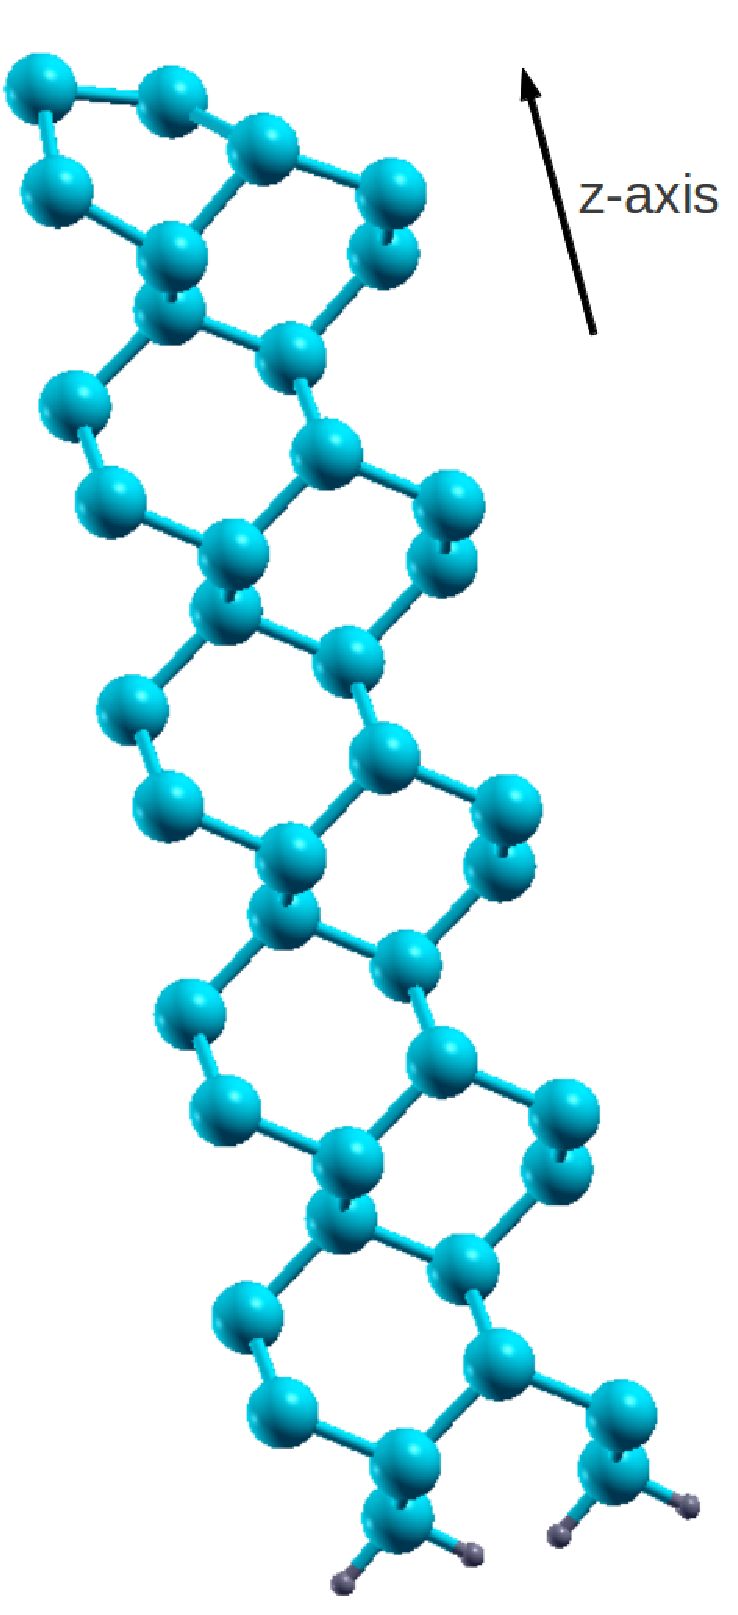
\includegraphics[scale=.3]{images/si2x1}
\caption{The slab shows a front clean Si(111)$2\times 1$ surface,
  while the back surface is ideally terminated Si bulk, where the
  dangling bonds are H (small balls) saturated. This picture shows 12
  Si layers and one H layer. 
\label{si2x1}} 
\end{figure}
The idea for such an slab is that the cristalline symmetry of the
H terminated surface imposes that $\chi^{\mathrm{H}}_{xxx}=0$, while
for the $2\times 1$ surface there is not such symmetry restriction and
then, $\chi^{2\times 1}_{xxx}\ne 0$.
Therefore, due to this fact, calculating $\chi_{xxx}$ for the full-slab
or the half-salb that contains the $2\times 1$ surface,
 ought to give the same result, since the contribution from the H
 saturated  surface is zero any way. Then, for this slab one must check
 whether or not this relation is satisfied,
\begin{align}\label{hs}
\chi^{\mathrm{half-slab}}_{xxx}(-2\go;\go,\go)
=
\chi^{\mathrm{full-slab}}_{xxx}(-2\go;\go,\go)
.
\end{align}
Indeed, in what follows we show the results of such a comparison.

The $2\times 1$ and the H surfaces are relaxed\textcolor{red}{Nicolas
  some details}, where we find agreement with previous results for
both surfaces.\cite{relax} For instance the Si-H bond distance is 1.48 $\AA$.
The calculation of the LDA is done using the ABINIT code with ???
pseudopotentials, that are of the BK form, and thus the $\bfv^\nl$
contribution can be calculated. We use the DP code for this end.
